\subsection{Predicci\'on en general}

Los modelos estadísticos se caracterizan por utilizar indicadores basados en el an\'alisis fundamental para escoger una cartera de acciones en un momento del pasado y evaluar su desempeño de acuerdo a los datos ya conocidos. Se enfocan en analizar tanto las acciones de valor como las acciones de crecimiento seg\'un la orientaci\'on de la investigaci\'on realizada. \\

\subsubsection{Acciones de valor}
% Value Investing: The Use of Historical Financial Statement Information to Separate Winners from Losers}

En el año 2000 Joseph Piotroski publica un artículo \cite{Piotroski2000} en el cual propone un modelo con el cuál se eligen acciones de valor (acciones con un bajo multiplicador entre su valor de mercado y el valor en libros) pero sin tomar en cuenta a las que tengan fundamentos pobres, con lo que obtiene rendimientos superiores al mercado. El proposito de discriminar según los fundamentos de la empresa es hallar acciones que esten subvaloradas y separarlas de las acciones que realmente tengan problemas financieros.\\

En su modelo, Piotroski utiliza nueve indicadores que reflejan tres áreas de la condición financiera de una empresa: rentabilidad, liquidez y eficiencia operativa. Clasifica a las firmas en diez portafolios dependiendo de las implicaciones de los indicadores con respecto a futuros precios y rentabilidad. Sus resultados indican la capacidad de la información contable de predecir el comportamiento futuro de una empresa y la demora del mercado en reconocer estos patrones predecibles.\\

Los nueve indicadores son:\\

\textbf{Retorno sobre activos (ROA)}: El ratio resultado de dividir el ingreso neto antes de ingresos extraordinarios sobre los activos. Si el resultado es positivo, eso indica que los los ingresos son positivos sin necesitar partidas extraordinarias por lo tanto el indicador $F\_ROA$ es 1, caso contrario es 0.\\

\textbf{Flujo de caja sobre activos}: El flujo de caja generado por el negocio en el periodo entre los activos. Si el resultado es positivo, eso indica que el flujo de efectivo es positivo por lo que el indicador $F\_CFO$  es 1, caso contrario es 0.\\

\textbf{Varianza retorno sobre activos}: Es el resultado de restar el retorno sobre activos del periodo anterior del retorno sobre activos actual, si el resultado es positivo significa que el retorno sobre activos se ha incrementado por lo que el indicador $F\_\Delta ROA$ es 1, caso contrario es 0.\\

\textbf{Ajustes (Accruals)}: Es el ingreso neto antes de partidas extraordinarias menos el flujo de caja de las operaciones, entre los activos.  Si el ingreso neto es mayor al flujo de caja debido a partidas extrardinarias, los estados financieros están siendo alterados para simular utilidades inexistentes. Si el resultado es positivo el indicador $F\_ACCRUAL$ es 1, caso contrario es 0.\\

\textbf{Varianza deuda de largo plazo}: Es el cambio en el ratio de la deuda de largo plazo entre los activos. Si el ratio baja de un periodo a otro eso señala que la deuda de largo plazo disminuye y por lo tanto el indicador $F\_\Delta LEVER$ es 1, caso contrario es 0.\\

\textbf{Varianza de la liquidez}: Este indicador mide el cambio en la liquidez de la empresa. La liquidez es la división de los activos l\'iquidos entre la deuda de corto plazo. Si la liquidez aumenta, es una buena noticia y el indicador $F\_\Delta LIQUID$ es 1, caso contrario es 0.\\

\textbf{Oferta de acciones}: Si la empresa emite acciones, es indicador de que no genera caja suficiente para financiar las actividades de la empresa. Si la empresa no emitió acciones, el indicador $EQ\_OFFER$ es 1, caso contrario es 0.\\

\textbf{Varianza del margen}: Es la variación del margen definido como el ingreso menos el costo de la operación entre el ingreso. Un incremento del margen indica aumento de la eficiencia, reducción de los costos de inventario o un aumento del precio del producto. Si el marge aumenta de un periodo a otro el indicador $F\_\Delta MARGIN$ es 1, caso contrario es cero. \\

\textbf{Varianza de la rotación de activos}: El ratio se define como las ventas totales entre los activos. Si aumenta el ratio, eso indica mayor productividad en la empresa y el indicador $F\_\Delta TURN$ es 1, caso contrario es 0.\\

Cada indicador es calificado de “bueno” o “malo” dependiendo de su impacto en la rentabilidad y precios futuros. La variable del indicador es uno si el indicador señala un impacto positivo en las utilidades o cero en caso contrario. La suma de todas las variables se acumula en la variable $F\_SCORE$, indicador agregado diseñado para medir la calidad de la posición financiera de una empresa,  mediante la ecuaci\'on \ref{Agregado F_SCORE}:\\

\begin{multline}
\label{Agregado F_SCORE}
F\_SCORE = F\_ROA + F\_\Delta ROA + F\_CFO + \\
F\_ACCRUAL + F\_\Delta MARGIN + F\_\Delta TURN + \\
F\_\Delta LEVER + F\_\Delta LIQUID + EQ\_OFFER \\
\end{multline}

La estrategia de inversión propone comprar las acciones cuyo $F\_SCORE$ sea alto y vender las que tengan un bajo resultado. Los resultados mostrados por el autor señalan un retorno promedio de 22\% en dos años de retener las acciones del ato $F\_SCORE$ y vender las de bajo $F\_SCORE$.\\

El aporte de este art\'iculo fue la creación de un modelo sencillo para invertir a largo plazo basándose en los fundamentos de las empresas. Utilizando las variables propuestas por Piotroski se han escrito otros artículos como los de Mohanram \cite{Mohanram2005} y Elleuch \cite{Elleuch2009}, quienes en sus respectivos paises (India y Tunez) utilizaron con \'exito el modelo de Piotroski.\\


%\subsubsection{Financial Statement Information, the Prediction of Book Return on Owners’ Equity and Market Efficiency: The Swedish Case}

El 2008, Stina Skogsvik \cite{Skogsvik2008} publica una investigación cuyo objetivo es probar si la Bolsa de Valores Sueca es eficiente con respecto a la información financiera disponible, con un enfoque en el mediano plazo.\\

A diferencia de investigaciones previas como la de Piotroski \cite{Piotroski2000}, el autor propone que utilizando solo el retorno sobre el capital (Return over Equity - ROE) es posible hacer pronósticos más acertados sobre las futuras ganancias de una empresa que utilizando el ROE en conjunto con otros ratios.\\

El valor de una empresa está determinada por el valor actual de utilidades futuras. De acuerdo con esta afirmación, la varianza del ROE indica si una empresa está disminuyendo o aumentando su valor debido a cambios en la cantidad de utilidades. Se considera para obtener la varianza un horizonte de tres años.\\

Al utilizar solo un indicador de rentabilidad, el autor sesga su estudio para favorecer los ingresos en el mediano plazo, sin tomar en cuenta otros indicadores que pueden señalar gastos extraordinarios que conllevaran mayores ingresos a futuro, como la ampliación de capacidad instalada o inversiones en investigación y desarrollo.\\


%\subsubsection{Fundamental Analysis Strategy and the Prediction of Stock Returns}

El 2009 el investigador tunecino Jaouida Elleuch \cite{Elleuch2009} examina una estrategia de inversión de análisis fundamental basada en el uso de información contable, para predecir ganancias con las acciones separando perdedores de ganadores, utilizando ratios contables basados en el análisis fundamental.\\

El art\'iculo se basa especialmente en el modelo de Piotroski \cite{Piotroski2000}, escoge 12 indicadores financieros seleccionados en base a su capacidad de predecir futuras ganancias. A cada indicador se le asigna cero o uno dependiendo si es negativo o positivo para el futuro de las utilidades de la empresa.\\

Los indicadores escogidos se diferencian del modelo de Piotroski \cite{Piotroski2000} en la consideraci\'on del inventario, las cuentas por cobrar y la productividad. Los indicadores propios del modelo Elleuch son:\\

\textbf{Variación Inventario}: Ratio que mide el porcentaje de cambio de las ventas entre el porcentaje de cambio en el inventario. Un incremento mayor del inventario es una mala señal ya que sugiere dificultades en la venta de las existencias. Si el inventario decrece, es una buena señal y el indicador es 1, caso contrario es 0.\\

\textbf{Variaci\'on Cuentas por cobrar}: Este indicador representa el porcentaje de cambio de las ventas menos el porcentaje de cambio de las cuentas por cobrar, ambos medidos respecto al periodo anterior. Un aumento en las cuentas por cobrar respecto a las ventas representa posibles problemas en el flujo de caja. Si el resultado es positivo es una buena señal y el indicador es 1, caso contrario es 0.\\

\textbf{Varianza Inversiones}: Este indicador mide el porcentaje de cambio en los gastos de capital entre el porcentaje de cambio en las ventas. La disminución es una mala señal que indica una gestión cortoplacista. Un valor positivo es una buena señal y el indicador es 1, caso contrario es 0.\\

\textbf{Utilidad Bruta}: Este indicador es el porcentaje de cambio en la utilidad bruta menos el el porcentaje de cambio en las ventas. Un decrecimiento de la utilidad bruta en relación a las ventas es mala señal. Como los estados financieros no necesariamente tienen ese dato, se puede utilizar el flujo de caja generado por la operación como sustituto. Un valor positivo es una buena señal y el indicador es 1, caso contrario es 0.\\

\textbf{Variaci\'n productividad por empleado}: Es el ratio definido por la variación de las ventas por empleado respecto al periodo anterior. Si aumenta es positivo y el indicador es 1, caso contrario vale 0.\\

Para probar el modelo, el autor compara el retorno obtenido por la cartera de acciones de alto F\_Score con el obtenido por la cartera de bajo F\_Score. Donde el retorno de una empresa es definido como el retorno de comprar y retener (buy-and-hold return BHR) obtenido en el periodo de tenencia que comienza al inicio del quinto mes posterior al cierre del año fiscal y que abarca los 15 meses posteriores. El retorno es calculado por la ecuaci\'on \ref{Calculo del retorno en un tiempo de tenencia}\\

\begin{equation}
\label{Calculo del retorno en un tiempo de tenencia}
\displaystyle BHR_{it} = \prod_{i=0}^{m} (1+R_{it})-1
\end{equation}

Donde $R_{it}$ es la tasa de retorno para la acción $i$ en la semana t. $m$ es el n\'umero de semanas en los 15 meses de tenencia de la acción.\\

El artículo utiliza el quinto mes porque asume que las empresas de Tunez publican sus estados financieros para esa fecha.\\
 
En las pruebas estadísticas realizadas, se demuestra que algunos indicadores tienen correlación negativa con el desempeño de la acción. Los indicadores Inversiones, apalancamiento (deuda de largo plazo) y las adquisiciones de activos fijos son presentados de forma negativa. Otros indicadores en cambio si consiguen altas correlaciones como el cambio en cuentas por cobrar, productividad de la fuerza de trabajo y retorno de los activos.\\


%\subsubsection{Fundamental Analysis and the Prediction of Earnings}

Los investigadores Dyna Seng y Jason R. Hancock en el 2012 \cite{DynaSeng2012}, buscan llevar el análisis fundamental más allá de los límites espacio temporales de estudios anteriores. Los autores critican a los trabajos previos por no dar suficiente importancia al contexto macroeconómico del país donde se ubican las empresas estudiadas.\\

La hipótesis de art\'iculo es que los indicadores fundamentales proporcionan información para predecir futuros cambios en las ganancias en el corto y largo plazo. A su vez, los indicadores contextuales y las condiciones macroeconómicas influyen en la capacidad de los indicadores fundamentales de predecir ganancias a futuro.\\

Para el an\'alisis fundamental toman en cuenta los nueve indicadores propuestos por Abarbanell y Bushee \cite{Abarbanell1998} y ejecutan tests para comprobar si los indicadores pueden tener influencia en las futuras ganancias y si las variables del contexto macroeconómico y del sector afectan el desempeño de los indicadores.\\

De los indicadores que utilizan, algunos como la variaci\'on del inventario, las cuentas por cobrar y las inversiones son compartidos con autores como Piotroski \cite{Piotroski2000}, Jaouida Elleuch \cite{Elleuch2009} y Meena Sharma y Preeti \cite{Preeti2009}, otras variables como los gastos de ventas, la tasa de impuestos, las auditorias contables y las variables de contexto son una propuesta original de los autores.\\

Las variables enfocadas en los estados financieros son las siguientes:

\begin{itemize}

\item \textbf{Ingresos brutos}: Este indicador se define como el resultado de restar el porcentaje de variación en en el margen (utilidad bruta entre ventas) al porcentaje de variación de las ventas.

\item \textbf{Gastos de ventas y administrativos}: Este indicador se define como el resultado de restar la variación porcentual de las ventas a la variación porcentual de los gastos de ventas y administrativos.

\item \textbf{Tasa de impuestos}: Este indicador se define como el porcentaje de los impuestos respecto al ingreso neto.

\item \textbf{Calidad de los ingresos}: Si se usa LIFO para el inventario el indicador es 0, 1 si es otro.

\item \textbf{Calificación del auditor}: Si el auditor no está calificado el indicador es 0, caso contrario es 1.
\end{itemize}

Los indicadores contextuales tomados en cuenta por los autores son:\\

\begin{itemize}

\item \textbf{Anuncios de ganancias}: Este factor se divide en buenas y malas noticias.

\item \textbf{Industria}: Manufactura, servicios, recursos naturales y comercio.

\item \textbf{Inflación}: Se considera inflación alta o baja.

\item \textbf{Crecimiento del PBI}: Se considera crecimiento alto o bajo.

\item \textbf{País de origen}: Se considera en EEUU o fuera de los Estados Unidos.

\end{itemize}

Los resultados obtenidos avalan la influencia de los indicadores fundamentales sobre las futuras ganancias, aunque en el corto plazo (un año) su confiabilidad es bastante mayor que en el largo plazo (cinco años).\\

%\subsubsection{Identifying Expectation Errors in Value/Glamour Strategies: A Fundamental Analysis Approach}

Joseph D. Piotroski y Eric C. So en el 2012 \cite{Piotroski2012}, critican la hipótesis de que las mayores ganancias se obtienen aceptando riesgos mayores. La hipótesis que postulan y demuestran en el art\'iculo es que las ganancias se obtienen tomando ventaja sobre las fallas del mercado, tal como estipula el an\'alisis fundamental desde Benjamin Graham \cite{BenjaminGraham2009}.\\

Los autores proponen una clasificación de las acciones en nueve cuadrantes determinados por dos indicadores: FSCORE (obtenido del modelo Piotroski \cite{Piotroski2000}) y el ratio Book to Market, el cual se obtiene dividiendo el valor de las acciones en libros entre en el valor de mercado. Esta clasificación se realiza para descubrir que acciones son las más rentables. Luego de obtener ambos datos sobre las acciones, se clasifican en una matriz dividida en alto, medio y bajo por cada uno, lo cual genera 9 secciones como se ve en la figura \ref{graf:matriz-valor-glamour} \cite{Piotroski2012}.\\

\begin{figure*}
   \centering
   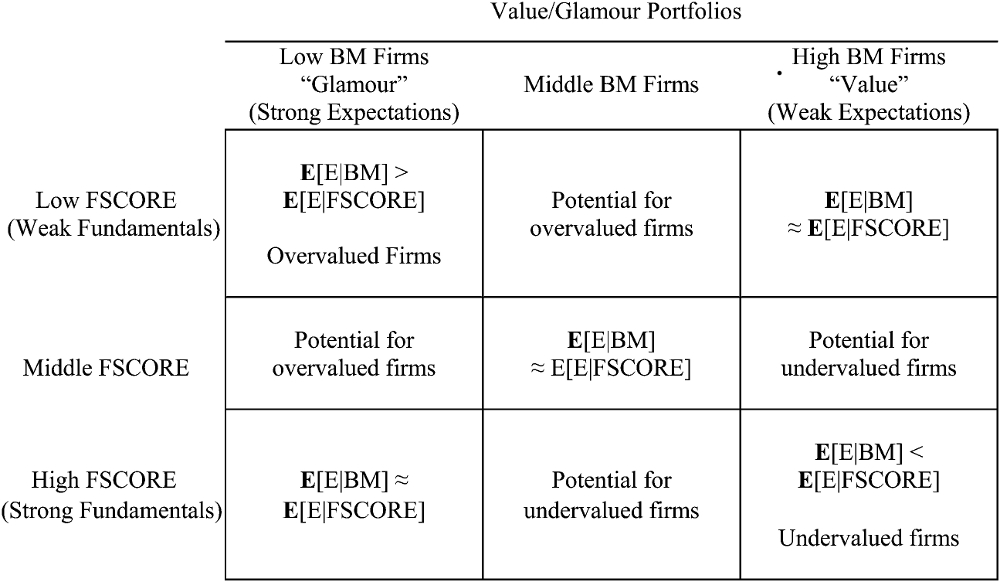
\includegraphics[scale=0.35]{imagenes/value_glamour_portfolio.jpg}
   \caption{Clasificaci\'on de las acciones \cite{Piotroski2012}}\label{graf:matriz-valor-glamour}
\end{figure*}

Una vez realizada la clasificación se llevan a cabo pruebas estadísticas para determinar en cual sector se obtienen mayores ganancias y comprobar si las hipótesis establecidas son correctas. Las pruebas se realizan con datos de las acciones de la Bolsa de Valores de Nueva York listadas en Compustat de los años 1970 al 2010 y dan como resultado un retorno de 22.64\% y 37.66\% para uno y dos años de inversión respectivamente en acciones subvaloradas.\\




\subsubsection{Acciones de crecimiento}

%\subsubsection{Separating Winners from Losers among Low Book-to-Market Stocks using Financial Statement Analysis}

Partha S. Mohanram, se basa en Piotroski y su modelo de indicadores pero se enfoca en las acciones de crecimiento (acciones cuyo valor de mercado tiene un alto múltiplo con respecto al valor en libros) en el artículo \cite{Mohanram2005} publicado el 2005. \\

Los indicadores utilizados por Mohanram se pueden dividir en tres: indicadores de rentabilidad y flujo de caja, de sobrevaloración en el mercado e indicadores de una contabilidad conservadora.\\

Dependiendo de que cada indicador sea positivo o negativo, se suma 1 o 0 a la variable GSCORE, a mayor GSCORE el autor considera más probable que la empresa de buenos rendimientos.\\

Los indicadores utilizados son iguales a los utilizados por Piotroski en lo que respecta a rentabilidad pero agrega nuevos indicadores que se basan en las expectativas del mercado y en identificar si la empresa se basa o no en una contabilidad conservadora.\\

\textbf{Indicadores relacionados a las expectativas del mercado.}\\

\textbf{Estabilidad de las utilidades}: Si la variabilidad de las utilidades es mayor a la variabilidad de las utilidades en empresas de bajo BM y del mismo sector económico, entonces G4 es 1, caso contrario, G4 es 0.\\

\textbf{Crecimiento de las ventas}: G5 es 1 si el porcentaje de crecimiento de las ventas es superior a las empresas de bajo BM en la misma industria, 0 en el caso contrario.\\

\textbf{Indicadores relativos a una contabilidad conservadora.}\\

\textbf{Inversión en R\&D}: G6 es 1 si el porcentaje de inversión de la empresa en R\&D es mayor al promedio de la industria y 0 en caso contrario.\\

\textbf{Gastos de capital}: G7 es 1 si el porcentaje de inversión de la empresa en gastos de capital es mayor al promedio de la industria y 0 en caso contrario.\\

\textbf{Inversión en publicidad}: G8 es 1 si el porcentaje de inversión de la empresa en publicidad es mayor al promedio de la industria y 0 en caso contrario.\\

Luego de pruebas estadísticas, el modelo demuestra ser más útil en identificar acciones perdedoras que acciones ganadoras, permitiendo al gestor de una cartera deshacerse de las acciones que producen las mayores pérdidas.\\

%\subsubsection{Prediction of stock returns for growth firms - a fundamental analysis}

El 2009, Meena Sharma y Preeti \cite{Preeti2009} examinan si el análisis fundamental, en forma de dos conjuntos de indicadores: tradicionales y de crecimiento, puede identificar a los mejores resultados cuando es aplicado a un portafolio de empresas con alto ratio PER.\\

El autor crítica que no se le de mayor importancia al crecimiento de una empresa en papers anteriores, debido a que las ganancias no se obtienen solo comprando valores cotizados bajo su valor intrínseco sino eligiendo empresas cuyo crecimiento va a superar al del mercado y por ende sus utilidades van a experimentar un rápido aumento.\\

La data es obtenida de La Bolsa de Valores de la India, entre los años 1998 y 2007. Las empresas de servicios no se toman en cuenta porque los ratios utilizados son intensivos en capital y debido a las conservadoras reglas contables, los activos intangibles son ignorados en los libros.\\

Los inversores dividen las acciones en dos tipos: de valor y crecimiento. Los inversores por valor buscan las acciones que se coticen a menos de su valor intrínseco, en cambio, los inversores de crecimiento buscan acciones de empresas cuyas perspectivas indican un rápido crecimiento.\\

Los ratios de valor considerados miden cuatro aspectos: rentabilidad, flujo de caja de la operación, eficiencia de la operación, liquidez y capacidad de generar caja, divididos en nueve indicadores y est\'an basados en el modelo Piostroski \cite{Piotroski2000}. Una variaci\'on  con respecto al trabajo de Piostroski es la utilizaci\'on de promedios del sector para compararlos con los diversos indicadores.\\

Los indicadores de valor que agregan Meena Sharma y Preeti son:\\

\textbf{Retorno sobre activos relativo (ROA-R)}: Si el retorno sobre activos, resultado de dividir el ingreso neto entre los activos, es superior al ROA promedio de la industria el indicador es 1, caso contrario es 0.\\

\textbf{Variación del margen}: Si el margen, definido como los ingresos netos sobre las ventas totales, es mayor al margen del año anterior, el indicador es 1, caso contrario es 0.\\

Para escoger los indicadores propios de las acciones de crecimiento, los autores se basan en Partha S. Mohanram \cite{Mohanram2005} y utilizan ratios orientados a medir el potencial de crecimiento miden cuatro aspectos, divididos en seis indicadores: volatilidad de las utilidades, estabilidad del crecimiento y gastos en investigación y desarrollo, capital y marketing. Los indicadores propios de los autores son aquellos miden la estabilidad del crecimiento.\\

\textbf{Volatilidad de las utilidades}: Se calcula midiendo la varianza de las utilidades de una empresa en los tres últimos años, luego se compara con otras empresas de crecimiento de la misma industria y si es menor que el promedio entonces el indicador es 1, caso contrario es 0.\\

\textbf{Estabilidad del crecimiento}: La volatilidad del crecimiento de las ventas es medida calculando la varianza del crecimiento de las ventas de la empresa en los últimos tres años. Si la volatilidad del crecimiento de ventas de la empresa es menor a otras empresas de crecimiento en la misma industria, el indicador es 1, caso contrario es 0.\\

\textbf{Crecimiento de las utilidades}: Si el crecimiento de las utilidades es superior al crecimiento de las ventas indica que mejora la eficiencia de la empresa y el indicador es 1, caso contrario es 0.\\

Los resultados obtenidos a base de pruebas estadísticas indican que el análisis fundamental basado en indicadores de crecimiento es exitoso en predecir que empresas van a desenvolverse mal en el futuro, permitiendo identificar a los perdedores.\\



\subsubsection{Aprendizaje de m\'aquinas}

%\subsubsection{An empirical methodology for developing stockmarket trading systems}

Adem\'as de los m\'etodos estad\'isticos, se ha automatizado el an\'alisis fundamental mediante aprendizaje de m\'aquinas (machine learning) utilizando los indicadores provistos por las investigaciones estad\'isticas para hallar patrones de comportaiento en los datos.\\

El 2009, Bruce J. Vanstone y Gavin Finnie \cite{Vanstone2009} esbozan una serie de pasos para crear redes neuronales orientadas a la inversión en los mercados de valores, utilizando el análisis fundamental o el análisis técnico y tomando en cuenta las principales restricciones a las que se verá sometida la red neuronal en el mundo real.\\

Los pasos para crear una red neuronal de predicción bursátil según los autores son:

\begin{itemize}
\item Elegir las variables adecuadas, ya sean indicadores fundamentales o de análisis técnico. Si el horizonte de tiempo es mediano o largo plazo (meses o años) se escogen los indicadores fundamentales y si es de corto plazo (días) se utiliza el análisis técnico. Se aconseja que se escojan indicadores avalados por estudios publicados.

\item Escoger las salidas de la red neuronal. Se recomienda sea solo una salida para impedir que diferentes salidas se obstruyan entre si al colocar los pesos en posiciones diferentes durante el entrenamiento.

\item Dividir la data disponible en data de entrenamiento y data de prueba. Se recomienda que la data se divida en un determinado punto del tiempo, de tal manera que los datos de toda acción queden divididos en data de entrenamiento y data de prueba. Esta distribución se debe a que los cambios en el tiempo afectan a todas las acciones, por lo que lo contrario implicaría conocer el futuro de un porcentaje de las acciones afectando el realismo de la predicción para las acciones de prueba. Se recomienda que los datos de entrenamiento sean un 80\% del total y se tenga por lo menos 10 años de datos para cada acción. Se debe incluir los datos de acciones que han salido de la bolsa para que la red neuronal se alimente de hechos reales.

\item Definir una función que sirva para evaluar la calidad de la salida de la red neuronal. En caso de inversión de largo plazo, se propone la fórmula \ref{Formula filtro}

\begin{multline}
\label{Formula filtro}
FilterSelectivity = \frac{ClosedTrades *100}{TotalTrades}
\end{multline}

Donde ClosedTrades es la cantidad de transacciones exitosas al alcanzar el porcentaje esperado de ganancia y TotalTrades es el total de transacciones realizadas.

\item Determinar la arquitectura de la red neuronal, para lo cual existen diversos enfoques que se recomienda investigar pero el artículo no elige uno sobre los demás.

\item Definir indicadores que señalen cuando se debe comprar y cuando vender.

\item Establecer límites mínimos de precio de las acciones. Si las acciones bajan de un límite mínimo, la red debe indicar que se venda.

\item Introducir restricciones del mundo real como las comisiones por operación, los impuestos, el capital disponible, la cantidad de acciones en venta, etc.
\end{itemize}

%\subsubsection{Stockmarket trading using fundamental variables and neural networks}

El 2010, Bruce Vanstone, Gavin Finnie y Tobias Hahn \cite{Vanstone2010} se basan en el modelo de Vanstone y Finnie del 2009 \cite{Vanstone2009} para crear redes neuronales orientadas al mercado de valores y utilizan las 4 variables fundamentales de Aby \textit{et al.} \cite{Aby2001} para conseguir retornos sobre el promedio del mercado en Australia.\\

Para elaborar la red neuronal se emplea data de la Bolsa de Valores de Australia (ASX200) desde 1994 al 2003 como entrenamiento y del 2004 al 2008 como prueba. En los datos de entrenamiento se incluyeron acciones que habían salido de la bolsa pero no se tomaron en cuenta para las pruebas.\\

Los valores que se escapaban de lo normal (bajo el 2.5\% o sobre el 97.5\% de la data) fueron eliminados de las series de datos para evitar problemas en el aprendizaje de la red neuronal. Las variables cuyos extremos fueron removidos son el ratio precio entre utilidades, retorno sobre el capital y porcentaje de pago de dividendos.\\

La red neuronal fue diseñada para producir una salida proporcional a los retornos esperados en el plazo de un año. El rango de la señal va de 1 a 100.\\


%\subsubsection{Implementing Value Investing Strategy by Artificial Neural Network}

El 2011, Kao-Yi Shen \cite{Shen2011} aplica el an\'alisis fundamental a la bolsa de Taiwan mediante una red neuronal artificial. Utiliza los indicadores de Piotroski \cite{Piotroski2000} para que la red neuronal aprenda a encontrar la relación entre los valores de los indicadores y el precio de la acción, identificando a las acciones subvaloradas por el mercado. El autor a su vez indica que hay realtivamente pocas investigaciones sobre la aplicaci\'on del an\'alisis fundamental utilizando algoritmos de aprendizaje de m\'aquinas.\\

La muestra utilizada en el artículo son las 400 compañias con la mayor relación entre su valor en libros y su valor de mercado (acciones de valor) sobre un total de 1200 empresas listadas en la bolsa de Taiwan a finales de Abril del 2009, por lo que los datos utilizados son del 2008. El tiempo de tenencia de las acciones, de 12 y 18 meses, es examinado para representar la salida de la red neuronal. Un cuarto de las acciones escogidas fue seleccionado al azar para servir de testeo. Para medir la variación se utilizo data del 2007.\\

El autor propone utilizar el modelo F-Score de Piotroski \cite{Piotroski2000}, reemplazando el indicador Activos Intangibles (Accruals) por Retorno del capital (ROE), mediante una red neuronal que aprenda de los valores periódicos de los indicadores y sea capaz de predecir hacia adelante.\\

El valor R es calculado dibujando la regresión lineal que mejor encaje entre las salidas de la red y sus metas como se ve en la Figura \ref{graf:regression-plot} \cite{Shen2011}, un indicador de la relación entre entradas y salidas. A más cercano a 1 sea, implica que la red neuronal genera mejores predicciones.\\

\begin{figure}[ht!]
   \centering
   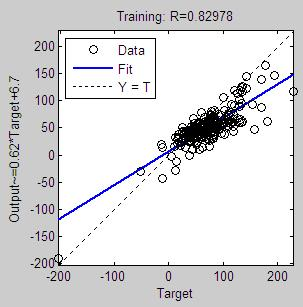
\includegraphics[scale=0.5]{imagenes/regression_plot.jpeg}
   \caption{Gráfico de la regresi\'on \cite{Shen2011}}\label{graf:regression-plot}
\end{figure}


La red neuronal consta de tres capas: entrada, oculta y salida. Luego de varias pruebas, el modelo de red neuronal que empleaba el algoritmo de Levenberg-Marquardt con un ratio de aprendizaje de 0.3 fue hallado como apropiado para la estructura de la red. En el estudio se encuentra que a más información histórica, mayor porcentaje de aciertos obtiene la red neuronal.\\

Una vez configurada la red, utilizan las 100 empresas que dejaron para pruebas para que la red neuronal genere 100 salidas (los tiempos de tenencia de 12 meses). Las salidas se ordenan de mayor a menor, representando la predicción de la red neuronal para los próximos 12 meses. El 30\% superior (las top 30) se comparó con los stocks disponibles en el mercado y se halló que la ganancia de 78.44\% era muy superior al mercado.\\